\documentclass{exam}
\usepackage{main}


\theoremstyle{definition}
\newtheorem{problem}{Problem}[section]

\theoremstyle{definition}
\newtheorem{definition}{Definition}[section]



\begin{document}

\title{
    {\Huge TJ IOI 2017}\\
    {\Huge Written Round}
}

\author{
	\large
	Thomas Jefferson High School for Science and Technology
}
\date{\large Saturday, May 13, 2017}

\pagenumbering{gobble}
\begin{titlepage}
    \maketitle
\end{titlepage}

% Before the actual contest
\pagenumbering{roman}

\tableofcontents
\newpage

\section*{Instructions}

This is the written round for the Thomas Jefferson Intermediate Olympiad in Informatics 2017.  This packet contains a series of written problems to be completed during the one ($1$) hour time period.  Once your time has expired, you are no longer permitted to write and must turn in all written solutions to a proctor.
\blank
During this round, you may not use \textbf{any external materials}, including all printed materials, and any electronic or communications devices. Any violation of this rule is grounds for immediate disqualification.
\blank
As a team, you may collaborate among each other. However, you may not communicate with any other teams during the contest window for any reason.
\blank
The style of pseudocode that you write for your solutions is not particularly important, as long as it is understandable. Feel free to use Java or Python syntax, if that's what makes the most sense to you. Note, however, that when we write pseudocode, we follow the convention that in the range $A \dots B$, $A$ is inclusive while $B$ is exclusive. This is equivalent to the Python convention for \verb|range(A, B)|.
\blank
Please use the zero-indexed convention when responding to questions. Responses that are one-indexed will not receive full credit.
\blank
You will write your answer to each problem on a blank sheet of paper. \textbf{You must write your team id on the top left hand corner of each page!}. If you fail to do so, your team will not receive credit for that problem. \textbf{Place the problem number at the top right hand corner of each page. Each problem should go on a separate sheet of paper. Feel free to ask your proctor for more paper if you need it.} 
\blank
\begin{center}
    \textbf{\Large Do not turn the page until instructed to do so.}
\end{center}

\newpage

% Begin the actual problems
\pagenumbering{arabic}



\section{Introduction}

One of the fundamental problems in computer science is sorting. Given a collection of items with a well-defined ordering, arrange them in order from ``lowest'' to ``highest''. Despite the problem's apparent simplicity, there are in fact a wide variety of algorithms used for sorting, each with different applications. In this round, we consider some of these algorithms, and explore their implementations and properties.

First, we begin with two important definitions, which are discussed extensively in the study guide. Both time complexity and space complexity are expressed using \textit{big O notation}.

\begin{definition}
    The \textit{asymptotic time complexity} of an algorithm is a measure of how the amount of time taken by an algorithm to run grows as a function of the input size. 
\end{definition}

\begin{definition}
    The \textit{asymptotic space complexity} of an algorithm is a measure of how the amount of memory required by an algorithm grows as a function of the input size. 
\end{definition} 

The following are two definitions of properties that can describe sorting algorithms, which we will discuss repeatedly throughout this round.

\begin{definition}
    A sorting algorithm is said to be \textit{stable} if and only if elements with the same key appear in the sorted array in the same order as they do in the input array. 
\end{definition}

\begin{definition}
    A sorting algorithm is said to be \textit{in-place} if and only if it uses a data structure with a sub-linear amount of extra space. 
\end{definition}



\begin{wrapfigure}{r}{0.20\textwidth}
    \centering
    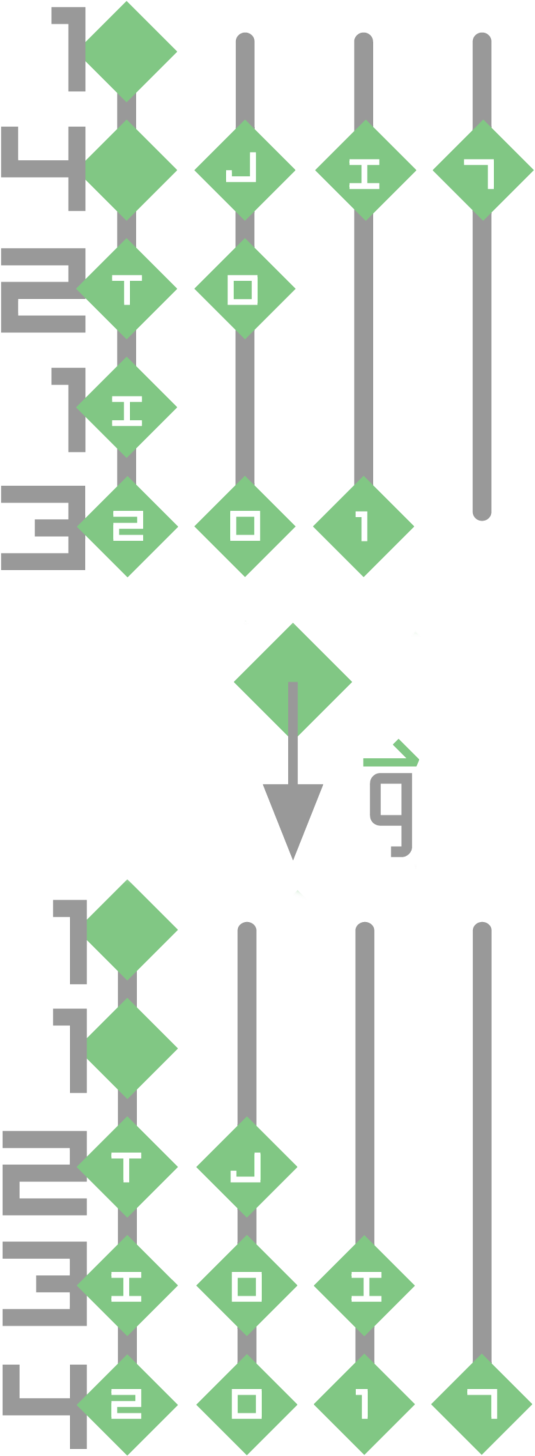
\includegraphics[width=0.17\textwidth]{tjioi_shirt_cropped.png}
    \label{fig:beadsort}
    \caption{The back of the TJ IOI shirt, depicting bead sort.}
\end{wrapfigure}

\section{Bead sort}

You may have observed an unconventional sorting algorithm on the back of your TJ IOI shirts, referred to as \textit{bead sort} or \textit{gravity sort}.

This algorithm uses the \textit{unary number system} to represent numbers. Although it is sometimes referred to as \textit{base-1}, it is in fact much simpler than other numerical systems: to represent the integer $ N $, we simply use $ N $ beads.

To start, we take the list of numbers we want to sort and place one in each row. We represent each number in each row by stacking the corresponding number of beads horizontally. To sort them, we let gravity do its work and allow the beads to fall, then count the beads in each row. We can then read off those counts to obtain the sorted list of numbers.

\begin{problem}[4 points]
    According to physics, the motion of a falling object that starts at rest is described by
    $$ \Delta y = -\frac{1}{2} g t^2 $$
    where $ g $ is the acceleration of gravity relative to Earth's surface. Explain why bead sort can be said to have a complexity of $ O(\sqrt{N}) $, where $ N $ is the number of integers to sort.
\end{problem}
%solving for t in the above equation, we get t = sqrt(2y/g). The max value of y is N, so t grows like sqrt(N) asymptotically. 

\begin{problem}[4 points]
    Despite its supposed $ O(\sqrt{N}) $ runtime, there are many issues that would prevent an actual implementation of bead sort from achieving such a runtime. 
    Explain why it is impossible to implement a sort that performs faster than $O(N)$ (without techniques such as parallel or quantum computing). 
\end{problem}
%It takes O(N) to position the beads in place OR
%we cannot guarantee that the array is sorted if we do not access every element at least once

%\begin{problem}[]
%   How much space does bead sort require? Is bead sort in-place? 
%\end{problem}
%O(N^2)

\begin{problem}[4 points]
    Besides questions about its complexity, bead sort is more limited than the other algorithms in this section, such as selection sort. Give an example of one such limitation.
\end{problem}
%only positive integers, cant sort strings, ...



\section{Elementary sorts}

From the study guide, you should already be familiar with at least two methods of sorting: \textit{selection sort} and \textit{insertion sort}. As you may know, both of these algorithms have a time complexity of $O(N^2)$.

Another property both of these algorithms share is that they are \textit{comparison-based sorts}. That is to say, we can implement them using only the following two operations.

\begin{itemize}
    \item A \textit{comparison} involves determining whether $ A[i] < A[j] $ in our ordering.
    \item An \textit{exchange} involves swapping the values of $ A[i] $ and $ A[j] $.
\end{itemize}

When we first discussed sorting, we said that a sort involves items with a well-defined ordering. In comparison-based sorts, this ordering is determined solely by the comparison function. There are nuances in the implementation of such a function, and several properties it must satisfy in order to sort correctly. However, in this section we will only consider sorting integers.


\subsection{Selection sort}

One of the simplest sorting algorithms, \textit{selection sort} operates by searching for each element amongst the items which have not yet been sorted, then placing it directly into its sorted position.

\begin{algorithm}[H]
\caption{Selection sort}
\begin{algorithmic}
\Function{SelectionSort}{$A$}
    \State $N \gets $ length of $A$
    \For {$i \in 0 \dots N$}
        \State $min \gets 0$
        \For{$j \in i+1 \dots N$}
            \If{$A[j] < A[min]$}
                \State $min \gets j$
            \EndIf
        \EndFor
        %\State $k$ \gets $getValueOfK()$ \Comment{Complete this for Problem \ref{problem:selection1}.}
        \State swap $ A[i] $ and $ A[min] $
    \EndFor
\EndFunction
\end{algorithmic}
\end{algorithm}

%\begin{problem} \label{problem:selection1}
%    Write pseudocode to determine the value of $ k $ above, so that the algorithm performs a sort.
%\end{problem}

\begin{problem}[4 points]
    %Selection sort can be implemented using only two types of operations: \textit{comparisons} (determine whether $ A[i] < A[j] $) and \textit{exchanges} (swap $ A[i] $ and $ A[j] $). As a result, we refer to it as a \textit{comparison-based sort}.
    Compute the number of comparisons and exchanges that the above algorithm performs on an array of length $ N $.
\end{problem}

\begin{problem}[4 points]
    Before every iteration of the loop, what do the values of $A[0 \dots i]$ represent, with respect to the original array? We can call this an \textit{invariant}, or a condition that must remain true.
\end{problem}

\begin{problem}[4 points]
    %\textit{Sort stability} is an important property of sorting algorithms, which states that if $ A[i] $ and $ A[j] $ are equal, then the ordering of $ i $ and $ j $ in the sorted array will be the same as their ordering in the initial array.
    Does the above algorithm result in a stable sort? If it is unstable, what would you change to make it stable?
\end{problem}



\subsection{Insertion sort}

Another algorithm is \textit{insertion sort}, which works by taking each element of the array, then shifting it into its sorted position amongst the items which have already been sorted.

\begin{algorithm}[H]
\caption{Insertion sort}
\begin{algorithmic}
\Function{InsertionSort}{$A$}
    \State $N \gets$ length of $A$
    \For{$i \in 1 \dots N$}
        \State $temp \gets A[i]$
        \State $k \gets i$
        \While{$k > 0$ and $A[k] < A[k-1]$}
            \State $A[k] \gets A[k - 1]$
            \State $k \gets k - 1$
        \EndWhile
        \State $A[k] \gets temp$
    \EndFor
\EndFunction
\end{algorithmic}
\end{algorithm}

\begin{problem}[4 points]
    What is the invariant that the algorithm maintains on $A[0 \dots i]$ before each time the main loop executes? Explain how this invariant differs from that in selection sort. How does this explain why $i$ starts at $1$ rather than $0$ as in selection sort?
\end{problem}

\begin{problem}[6 points]
    We stated above that insertion sort was a comparison-based sort. However, the implementation shown here is written in terms of array accesses. Re-write the loop of the algorithm to use only compare and exchange operations.
\end{problem}

\begin{problem}[8 points]
    Unlike selection sort, the number of operations performed by insertion sort depends on the data. Calculate the minimum and maximum number of comparisons and exchanges when sorting an array of length $N$, and describe under what conditions they are achieved.
\end{problem}

\begin{problem}[4 points]
    Compare the number of comparisons and exchanges performed using selection sort and insertion sort. Under what conditions does insertion sort perform more or less comparisons than selection sort?
\end{problem}



\section{Linearithmic sorts}

In order to improve the running time complexity of elementary sorts, we can use the \textit{Divide and Conquer} algorithm paradigm. All divide and conquer algorithms consist of three parts: 

\begin{enumerate}
    \item \textit{Divide:} divide the problem into two sub-problems
    \item \textit{Conquer:} recursively solve each sub-problem
    \item \textit{Combine:} combine the solutions of each sub-problem into a single solution
\end{enumerate}



\subsection{Merge sort}

In merge sort, we divide the problem into two sub-problems of equal size. The obvious way to accomplish this is to simply divide the input array into the first and second half at the midpoint of the array, which is constant time. We then recursively sort each half, and then merge the two sorted half-arrays into a single sorted array. The pseudocode below outlines this process. 

\begin{algorithm}[H]
\caption{Merge sort}
\begin{algorithmic}
\Function{MergeSort}{$A$}
    \State $ mid \gets N/2$
    \State \Call{MergeSort}{$A[0 \dots mid]$}
    \State \Call{MergeSort}{$A[mid \dots N]$}
    \State \Return \Call{merge}{$A[0 \dots mid]$, $A[mid \dots N]$}
\EndFunction
\Function{Merge}{$A$, $B$}
    \State $//$ Your code here \Comment{refer to problem \problemref{4.1}}
\EndFunction
\end{algorithmic}
\end{algorithm}


\begin{problem}[8 points]
    Write the pseudocode for the merging procedure. Your pseudocode should be a function called "merge" that takes two sorted arrays as input and outputs a single, sorted array whose length is the sum of the length of the input arrays. Your implementation of the merging procedure must run in $O(N)$ or better. 
\end{problem}

\begin{problem}[4 points]
    What is the space complexity of the merging procedure? Is it in-place? 
\end{problem}

In the next three problems, we will show that the runtime complexity of merge sort is $O(N \log N)$. A common technique when trying to prove the time complexity of divide and conquer algorithms is to use the technique of  \textit{mathematical induction}. The basic premise of mathematical induction is to show that $(1)$ the result holds for a base case, and that $(2)$ if the result holds for a smaller case, then it must also hold for a larger case. The latter of these two steps is called the \textit{inductive step}.

Essentially, a proof by induction creates a ``snowball effect'', where if a statement holds for some natural number, then it must hold for all natural numbers by the inductive step. The base case for merge sort occurs when $N = 1$ and clearly runs in constant time.

\begin{problem}[6 points]
    Let $ T(N) $ be the number of comparisons needed to sort an array of size $ N $. Show that 
    \begin{equation}
         T(N) = 2 T\left(\frac{N}{2}\right) + O(N)
    \end{equation}
\end{problem}

\begin{problem}[8 points]
    Assume that $ T(\frac{N}{2}) = \frac{N}{2} \log \frac{N}{2} $. This is known as our inductive hypothesis. Show that $ T(N) = O(N \log N) $ by substituting the expression into equation $(1)$. 
\end{problem}

\begin{problem}[4 pionts]
    Our proof appears to only account for $N$ that are powers of two. Explain why we can generalize this result to hold for all positive integers $N$. 
\end{problem}



\section{Radix Sort}

Elementary sorts, merge sort, and quick sort are also known as \textit{comparison-based sorts} because they repeatedly compare two elements of the list to determine the final sorted array. It can be proven that comparison-based sorts have a lower bound worst-case time complexity of $O(N \log N)$. That is, no comparison-based sort is guaranteed to always run faster than $O(N \log N)$. In this section, we consider how we can sort lists without directly comparing any two elements. 



\subsection{Key-Indexed Sorting}

Consider the following problem: Kevin has a list of all students at TJHSST. Each student has a name, and a grade level. Kevin wants to sort the students by their grade level: 9th, 10th, 11th, and 12th. Help Kevin do this.

Although we could use a comparison-based sorting algorithm, it's not hard to imagine an even simpler solution: create one dynamic array for each grade level; place the students into the array corresponding to their grade level; then merge them back into the original array.

To avoid the overhead of dynamic arrays, we can do this with only one auxiliary array of the same size. To do this, we first need to determine where we will put the 9th graders in the auxiliary array; and where we will put the 10th, 11th, and 12th graders. 

Notice, though, that in the auxiliary array, all 10th graders must occur after all 9th graders, all 11th graders must occur after all 9th and 10th graders, and all 12th graders must occur after all 9th, 10th, and 11th graders. This motivates us the count the frequency of each grade level so that we can compute their range of possible indices. 

\begin{problem}[4 points]
    Write pseudocode to count the number of students in each grade. Your pseudocode should be a function that takes an integer array as input and outputs an integer array of length four. The contents of the input array consists entirely of 9, 10, 11, and 12. The first entry of the output array should be the number of 9th graders, the second the number of 10th graders, and third the number of 11th graders, and the fourth the number of 12th graders. 
\end{problem}

\begin{problem}[4 points]
    Supposed that the number of 9th, 10th, 11th, and 12th graders are $c_{1}$, $c_{2}$, $c_{3}$, and $c_{4}$ respectively. What are the bounds on possible indices for 9th, 10th, 11th, and 12th graders in the auxiliary array? (In other words, between which two indices must all 9th graders be in the auxiliary array, and same for 10th, 11th, and 12th graders?)
\end{problem}

\begin{problem}[6 points]
    Based on your response to problem \problemref{4.2}, write pseudocode to sort the 9th, 10th, 11th, and 12th graders using key-indexed sorting. Your pseudocode should be a function that takes as input an integer array and outputs an integer array. Each entry in the input array is either a 9, 10, 11, or 12. The output array should be the input array in sorted order. Your code may call the function KeyIndexSort and assume that it works correctly, regardless of whether your solution to problem \problemref{5.1} is correct. 
\end{problem} 

\begin{problem}[8 points]
    For most problems, however, we are required to sort items into more than just four categories. Generalize your algorithm in problem \problemref{4.3} so that it sorts an array of $R$ different values using key-indexed sorting. $R$, the number of unique keys (or ``digits''), is known as the \textit{Radix}. Your pseudocode should be a function that takes as input an integer array and integer $R$, and outputs an integer array. The input array should consist of integers between $0$ and $R-1$, and the output array should be the input array in sorted order. 
\end{problem}


\begin{problem}[4 points]
    What is the time complexity of key-indexed sorting?
\end{problem}

\begin{problem}[4 points]
    What is the space complexity of key-indexed sorting. Is it in-place? 
\end{problem}

\begin{problem}[8 points]
    Prove that key-indexed sorting is stable. A semi-rigorous argument can be enough to get full credit. 
\end{problem}



\subsection{Sorting Strings}


\begin{figure}[h]
\begin{center}
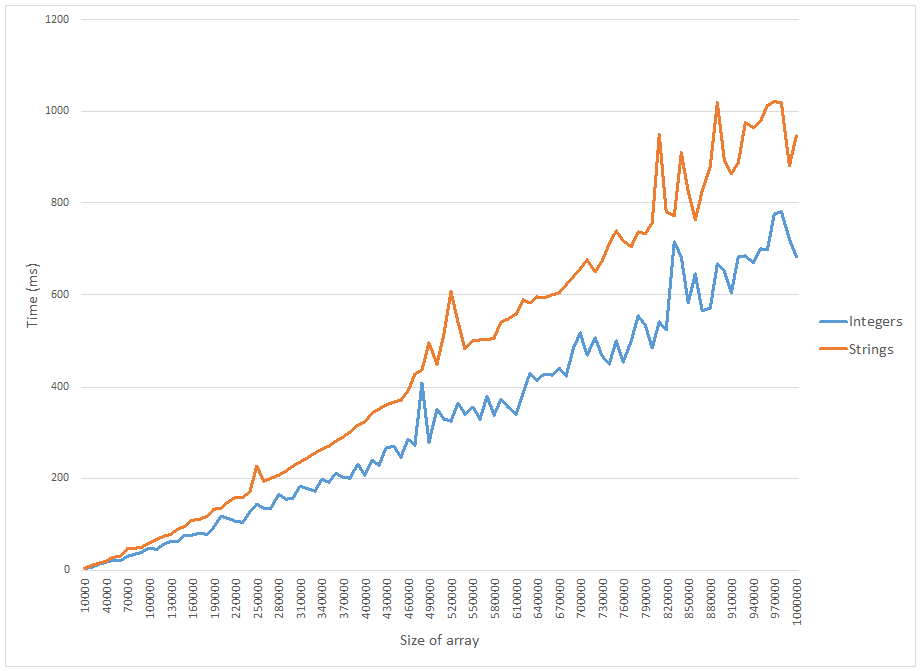
\includegraphics[width=0.6\textwidth]{chart1.png} \\
\label{fig:mergesort}
\caption{Merge sort on integers and strings. }
\end{center}
\end{figure}


\begin{problem}[6 points]
    Previously, we considered comparison-based sorts, which we used to sort integers in $ O(N \log N) $ time.
    The above graph shows the results of using merge sort to sort integers and strings of length 10.
    Give an explanation for why sorting strings takes significantly longer than sorting integers. What is the runtime complexity of sorting $N$ strings, each with length up to $K$?
\end{problem}

In order to speed up string sorting, we would like to apply key-indexed sorting. However, it is not immediately apparent how we can ``bucket'' strings into a constant number of keys. We can, however, use key-indexed sorting to sort characters (since each of the 128 different ASCII characters can act as an individual key). The following two algorithms describe two different approaches how how key-indexed sorting can be used to sort strings. 



\subsection{Least Significant Digit Radix Sort}

In problem 4.5, we showed that key-indexed sorting is stable, which means that $a$ came before $b$ in the original array and have equal keys, then $a$ must come before $b$ in the sorted array. In other words, keys with equivalent keys must retain their original relative ordering. 

Suppose that we wanted to sort strings of length 2. Since key-indexed sorting is stable, we can first sort the strings keyed by the second character (or digit), and then sort them again keyed by the first digit. We can also extend this to strings of length 3 by sorting by the third, then second, then first digit. This sorting algorithm is called Least Significant Digit Radix Sort because we key index sort from the least to most significant digit (or from right to left). 


\begin{algorithm}[H]
\caption{LSD Radix Sort}
\begin{algorithmic}
\Function{LSDRadixSort}{$A$}
    \State $ buffer \gets $ empty array of size equal to A's size
    \State $index \gets R-1$
    \While{$index \geq 0$}
        \State \Call{KeyIndexSort}{$A$, $index$, $buffer$}
        \State $ index \gets index - 1 $
        \State \Call{copy}{$A$, $B$}
    \EndWhile
    \State \Return $A$
\EndFunction
\end{algorithmic}
\end{algorithm}


\begin{problem}[8 points]
    Given a list of 15 strings of length 4, sort the strings by tracing through Algorithm 3. Write down the contents of the array after each call of KeyIndexSort. 
    \begin{verbatim}
BEAD
AAEB
BADA
EBAC
BECE
ECAD
BECC
ACAC
CBDD
DECD
CADD
EEAA
CABB
AADE
ACAC
    \end{verbatim}
\end{problem}

\begin{problem}[6 points]
    We will now show that LSD Radix Sort is correct for strings of any length using induction. Assume that we are able to sort strings of length $k$ using LSD Radix Sort. Show that this implies that we can also sort strings of length $k+1$ using LSD Radix Sort. 
\end{problem}

\begin{problem}[4 points]
    Prove that LSD Radix Sort is $O(MN)$, where $M$ is the length of the longest string.
\end{problem}

\begin{problem}[4 points]
    Is LSD Radix Sort stable? If yes, explain why. If not, give a counterexample. 
\end{problem}

\begin{problem}[8 points]
    (a) Explain (and give an example) of why key-indexed sorting from right to left will not work if we need to sort strings of different length (4 points).
    (b) Explain how LSD Radix Sort can be used to sort a list of strings if not all strings are of the same length (4 points). 
\end{problem}

\begin{problem}[6 points]
    Above, we used LSD Radix Sort to sort strings with an alphabet of 128 ASCII characters. Explain how LSD Radix Sort can be used to sort a list of 64-bit unsigned integers.
\end{problem}

\begin{problem}[6 points]
    Although LSD Radix Sort has a better big-O complexity than Quicksort and Merge sort ($O(N)$ vs. $O(N \log N)$), it sometimes performs slower. Explain why this might be the case. (Hint: What aspect of the actual time complexity does big-O notation not tell us?) 
\end{problem}



\subsection{Most Significant Digit Radix Sort}

In order to circumvent the problem of sorting strings with different lengths, we can instead process the characters from left to right, or from most to least significant digit. Note, however, that we can no longer key-index sort the whole list of strings from keyed by characters from left to right like in LSD Radix Sort since the resulting array would no longer be sorted correctly.

In order to make sure successive key-index sorts do not perturb the ordering of the first character, we must instead separately sort each group of strings with matching first characters using key-indexed sort keyed by the second character. In other words, we follow a procedure similar to the divide-and-conquer paradigm: the first key-indexed sort splits up our original problem into $R$ subproblems, where $R$ is the alphabet size. We then solve each of those subproblems recursively. We can then repeat this process from left to right, yielding an algorithm know as Most Significant Digit Radix Sort.


\begin{problem}[10 points]
    Write the pseudocode for MSD Radix Sort. Your pseudocode should be a function that takes a string array as input and outputs a string array. Your functin  may call a recursive helper-function if necessary. 
\end{problem}

\begin{problem}[8 points]
    Given 15 strings of arbitrary length at most 5, sort the strings by tracing through MSD Radix Sort. Write down the contents of the array after each key-index sort. 
    \begin{verbatim}
EDACD
BD
EDCEB
EDCA
EBE
E
DCCA
AEEAB
DDCD
ECCBA
AEEA
DAB
EABA
ECCA
EDC
    \end{verbatim}
\end{problem}

\begin{problem}[8 points]
    What is the worst-case number of array accesses that MSD performs? What about the best case? In your answer you may refer to $W$ as the length of the longest string. 
\end{problem}

\begin{problem}[4 points]
    Explain why on average, MSD takes less time than LSD.
\end{problem}

\begin{problem}[8 points]
    Explain bead sort in terms of Radix Sort. One reason for its supposed speed is that the beads in each column are permitted to fall simultaneously and independently. Why can we do this with bead sort, but not with LSD or MSD?
\end{problem}


\end{document}
